% AOSD report template
% Jakub Perdek 2020

%\documentclass[11pt,english,a4paper,twoside]{article}
\documentclass[11pt,slovak,a4paper,twoside]{article}



\usepackage[slovak]{babel}
\usepackage[utf8]{inputenc}
\usepackage[T1]{fontenc}

\usepackage{url}
\usepackage[nottoc]{tocbibind}
\usepackage{ifthen}
\usepackage{float}
\usepackage[hidelinks]{hyperref}
\usepackage{graphicx}
\usepackage{listings}


\newcommand{\magnf}{.65}
\newcommand{\codesize}{\footnotesize}
\newcommand{\lsti}{\ajset\lstinline[basicstyle=\fontsize{10}{12}\selectfont]}
\newcommand{\emp}[1]{\emph{#1}}
\newcommand{\ffe}[1]{\textsf{#1}}

% balík listings niekedy niektoré kľúčové slová nezvýrazňuje ak to nedostane príkazom tesne pred textom
\newcommand{\ajset}{\lstset{emph={class,aspect,new,call,execution,set,int,advice,public,thisJoinPointStaticPart,thisEnclosingJoinPointStaticPart,@annotation,dominates},emphstyle=\bfseries}}

\newcommand{\reporttitle}{Aspektovo riadená konfigurácia radu softvérových výrobkov} % here goes your fancy title

\pagestyle{myheadings}
\markboth{\reporttitle}{Kvalita refaktorovaného kódu, modulárnosť a derivovanie produktov 2021/22, FIIT STU}

\title{\reporttitle}

\author{Jakub Perdek} % your name

\date{In\v{s}titút informatiky, informa\v{c}ných systémov a softvérového in\v{z}inierstva\\
      Fakulta informatiky a informa\v{c}ných technológií\\
      Slovenská technická univerzita v Bratislave\\[6pt]
      20. Október, 2021} % modify the date if different



\begin{document}

\maketitle

\begin{abstract}
Generovanie variantov produktov pomáha vytvori\v{t} produkty z danej domény efektívnej\v{s}ie a lacnej\v{s}ie. Nevzniká tak iba jeden produkt, ale \v{l}ahko adaptovate\v{l}né produkty pre rôzne prostredia, jazyky a \v{d}al\v{s}ie po\v{z}iadavky (Beuche a Dalgarno 2006). Derivova\v{t} produkty prispôsobené po\v{z}adovanej variabilite mo\v{z}no za pomoci aspektovo orientovaného prístupu, hlavne jazyka AspectJ  \cite{young_using_1999} (Young a Math, 1999), ktorého mo\v{z}nosti by sme chceli pri tejto úlohe preskúma\v{t}. Vyberáme pou\v{z}itie jazyka AspectJ, preto\v{z}e umo\v{z}\v{n}uje oddeli\v{t} zále\v{z}itosti ako je logovanie, ke\v{s}ovanie, poolovanie, ale hlavne je mo\v{z}né vyradi\v{t} z vykonávania vybrané aspekty, respektíve isté vlastnosti aplikácie, prípadne aj celkovú závislos\v{t} na tomto jazyku \cite{laddad_aspectj_2003} (Laddad, 2003).												

Zaujíma nás preto uplatnenie jazyka pri umo\v{z}není konfigurovate\v{l}nosti konkrétnych vlastností v kóde, a samotné generovanie konkrétneho variantu produktu s prípadnou po\v{z}iadavkou nezávislosti implementácie od tohto pou\v{z}itého jazyka. Zhodnotíme prínosy a kvality aspektovo orientovaného prístupu na konkrétnej implementácii, a porovnáme ich s identifikovanými problémami a benefitmi spomenutými v rôznych reimplementáciách u\v{z} existujúcich softvérových systémov ako je vedecká kalkula\v{c}ka (Botterweck, 2009) alebo databázový systém (Kastner, 2007). Samotné analýzy nazna\v{c}ujú význam vo\v{l}by domény pri zostrojovaní radu softvérových produktov, preto by sme v neposlednom rade chceli porovnať vplyv domény pri ich implementácii.								

Plánujeme prispôsobi\v{t} existujúcu hru Battleship tak, aby umo\v{z}\v{n}ovala mana\v{z}ova\v{t} vlastnosti na základe u\v{z} vytvoreného modelu vlastností, vä\v{c}\v{s}ina ktorých nie je vôbec implementovaná. Cie\v{l}om je aj analyzova\v{t} spôsoby odvodenia konkrétneho produktu, a mieru jeho závislostí od jazyka AspectJ. 								

\v{D}al\v{s}ou aplikáciou pre analýzu je odvodzovanie rôznych fraktálov (uká\v{z}ky typov nájdete v Pelánek, 2012) z pôvodného algoritmu, ktoré by sme realizovali zásahom aspektov do jeho vykonávania. Predpokladáme, \v{z}e úloha samotného návrhu vlastností pre uvedenú aplikáciu je ur\v{c}ená hodnotou vzh\v{l}adu fraktálu, pri\v{c}om zhotovenie radu produktov pre\v{n} mô\v{z}e vy\v{z}adova\v{t} iné nároky na model vlastností, ako napríklad generovanie v\v{s}etkých mo\v{z}ných derivácií pre následné overenie estetiky a identifikovanie najvhodnej\v{s}ích kandidátov. Zamý\v{s}\v{l}ame preto zhodnoti\v{t} význam prípadného potenciálu aspektovo orientovaného rie\v{s}enia pre derivovanie konkrétnych fraktálov.
\end{abstract}


\section{Úvod} \label{in}



\begin{enumerate}

	\item \v{C}o najva\v{c}\v{s}í po\v{c}et vyu\v{z}ití u\v{z} prítomných rozhraní jednotlivých komponentov implementujúcich návrhový vzor Strategy a vyu\v{z}ívajúcich reflexiu (nie je v diagrame komponentov znázornené).

	\item \v{C}o najmen\v{s}í po\v{c}et závislostí medzi jednotlivými komponentmi.

	\item Jednoduché vyu\v{z}itie iného komponentu v rámci druhého komponentu bez nutnosti vytvára\v{t} rozhrania týchto komponentov.
	
	\item Zahrnú\v{t} dôle\v{z}ité technológie a vhodne ich rozdeli\v{t} do komponentov. 
	
	\item Oddeli\v{t} konkrétnu implementáciu hry od herného engínu ako dôkaz znovupou\v{z}ite\v{l}nosti herného engínu. 
	
	\item Zahrnú\v{t} dôle\v{z}ité technológie a vhodne ich rozdeli\v{t} do komponentov. 
	
	\item Navrhnú\v{t} komponent prepájajúci podstatné \v{c}asti herného engínu, aby kód v pou\v{z}ívate\v{l}ovom komponente pracujúci s engínom bol \v{c}o naj\-jednoduch\v{s}í.
	
\end{enumerate}
  

\section{Preh\v{l}ad obsahu sekcií} \label{content}

Sekcia~\ref{insight} poskytuje charakteristiku jadra herného engínu a popisuje rozdiely medzi ním a samostatnou hrou.
Sekcia~\ref{analysis} sa zameriava na analýzu architektúry herného engínu na základe kódu, ktorý obsahuje. Triedy a vz\v{t}ahy medzi nimi znázor\v{n}ujeme pomocou nami vytvoreného diagramu tried. Vytvorený diagram balíkov by mal znázor\v{n}ova\v{t} vz\v{t}ahy medzi balíkmi.  
V sekcii~\ref{layersSection} pri analýze \v{s}truktúry rozde\v{l}ujeme monolyt na jednotlivé vrstvy. V tejto \v{c}asti sa sna\v{z}íme o realizáciu komunikácie len v rámci susedných vrstiev. Dosiahnu\v{t} komunikáciu len v jednom smere je vítané.
V sekcii~\ref{engineAsSubsystem} sa sna\v{z}íme oddeli\v{t} herný engín od hry u\v{z} v samotnom návrhu tým, \v{z}e z engínu vytvárame predpripravený subsystém, ktorý mô\v{z}e by\v{t} v prípade potreby nakonfigurovaný pod\v{l}a potrieb hry. Tvorba hier by preto mala by\v{t} jednoduch\v{s}ia a prepojenia s engínom by mali by\v{t} v men\v{s}om po\v{c}te. 
Sekcia~\ref{distributedSOA} reprezentuje návrh distributívneho rie\v{s}enia pre lep\v{s}iu roz\v{s}írite\v{l}nos\v{t} a tvorbu modulov. SOA by mala byť univerzálnou vo\v{l}bou kvôli princípu vo\v{l}nej väzby pri skladaní slu\v{z}ieb, ale distributívna architektúra zalo\v{z}ená na vzdialenom volaní procedúry mô\v{z}e by\v{t} rýchlej\v{s}ia. V tejto \v{c}asti sa zameriavame hlavne na zmen\v{s}enie závislostí medzi 3D matematikou.
Sekcia~\ref{applicationJavascript} je venovaná realizácii engínu v jazyku Javascript. Sna\v{z}íme sa poskytnú\v{t} informácie o pou\v{z}ití podobnej technológie zalo\v{z}enej na funkcionalite plátna. Zaoberáme sa komplikáciami a implikáciami preneseného rie\v{s}enia v súvislosti s architektúrou.
Sekcia~\ref{eval} zhodnocuje vykonanú prácu spolu s opisom hlavných prínosov jednotlivých \v{c}astí rie\v{s}enia.
Sekcia~\ref{recentwork} sumarizuje preh\v{l}ad \v{d}al\v{s}ích publikácií a vývoja podobných herných engínov. Cie\v{l}om je poskytnú\v{t} aj informácie o \v{d}al\v{s}ích komponentoch a technológiách pri tvorbe jadra herného engínu softvérového rie\v{s}enia.
Sekcia~\ref{cc} obsahuje zhodnotenie práce a \v{d}al\v{s}ích mo\v{z}ností roz\v{s}írenia tejto práce.


\section{Rad softvérových výrobkov a analýza domény} \label{insight}


\section{Aktuálny stav a návrh riešenia pre hru Battleship} \label{analysis}


\begin{figure}[H]  %vycentrovany obrazok grafu, vsadeny do odstavca
					\begin{center}
									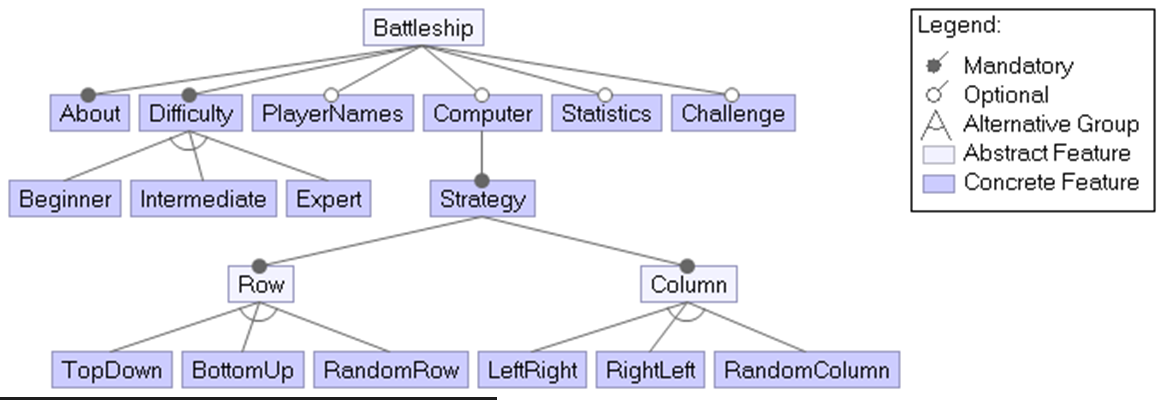
\includegraphics[width=\linewidth]{fig/battleshipFeatureModel.png}
									\caption{Diagram vlastností pre hru Battleship}
									\label{battleshipFeatureModel}
					\end{center}
\end{figure}

\section{Úprava hry Battleship s použitím jazyka AspectJ} \label{analysis}

\begin{figure}[H]  %vycentrovany obrazok grafu, vsadeny do odstavca
					\begin{center}
									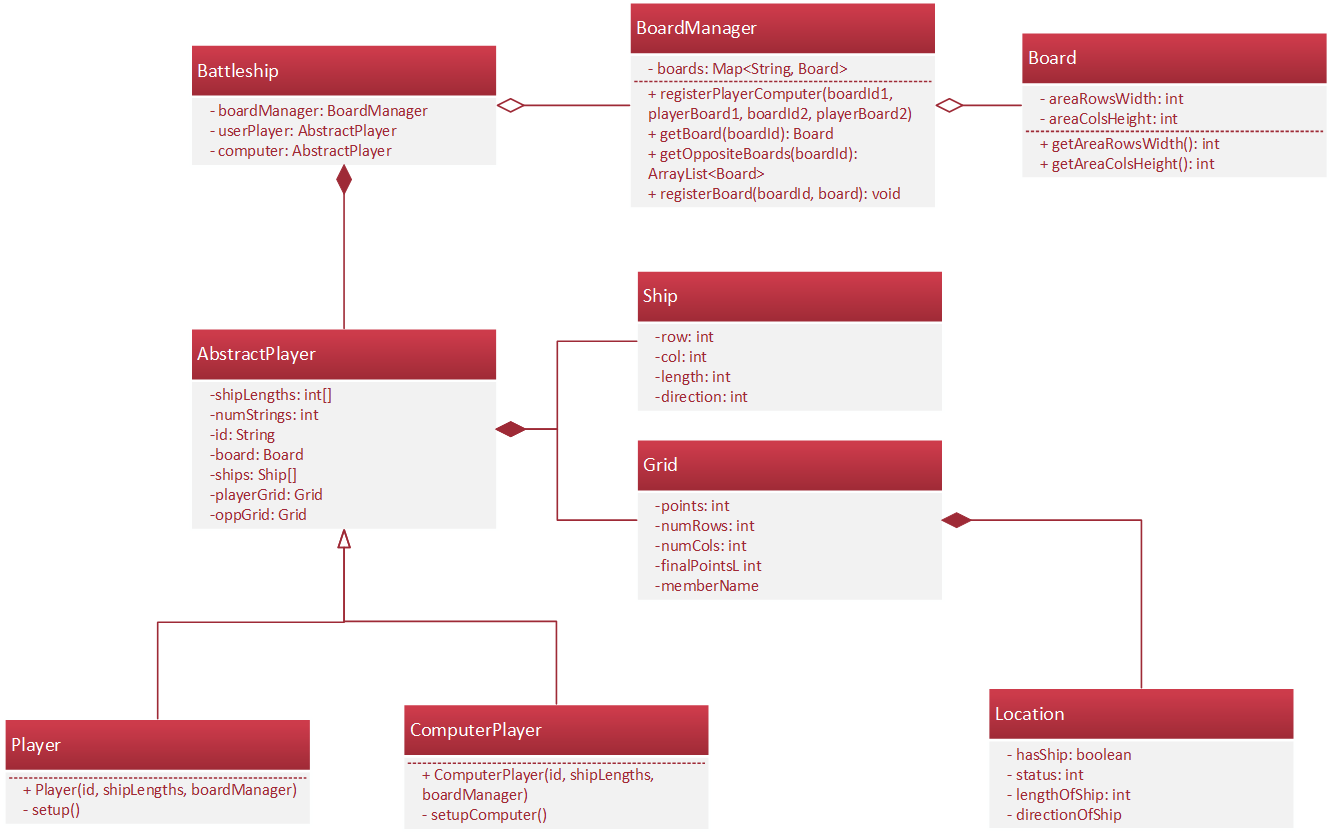
\includegraphics[width=\linewidth]{fig/refactoredSchema.png}
									\caption{Diagram tried upraveného riešenia}
									\label{refactoredSchema}
					\end{center}
\end{figure}


\begin{figure}[H]  %vycentrovany obrazok grafu, vsadeny do odstavca
					\begin{center}
									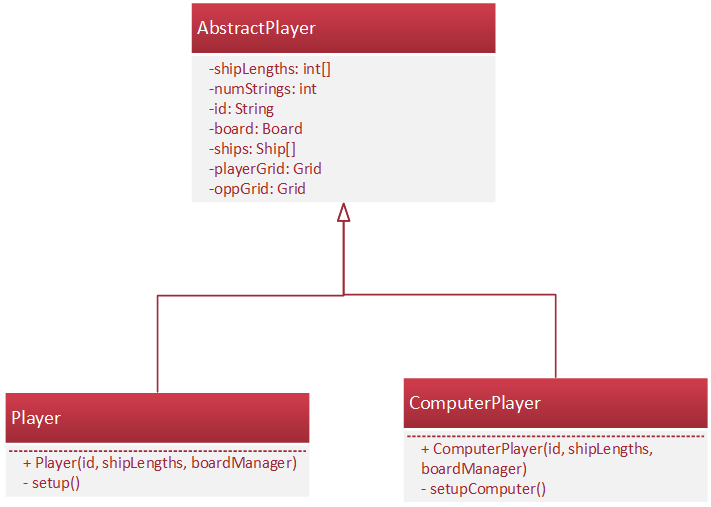
\includegraphics[height=10cm]{fig/playerAbstraction.png}
									\caption{Abstrakcia hráča}
									\label{playerAbstraction}
					\end{center}
\end{figure}

Po prvej iterácii je diagram balíkov zobrazený na obrázku \ref{problemsOfAspectJ}.

\begin{figure}[H]  %vycentrovany obrazok grafu, vsadeny do odstavca
					\begin{center}
									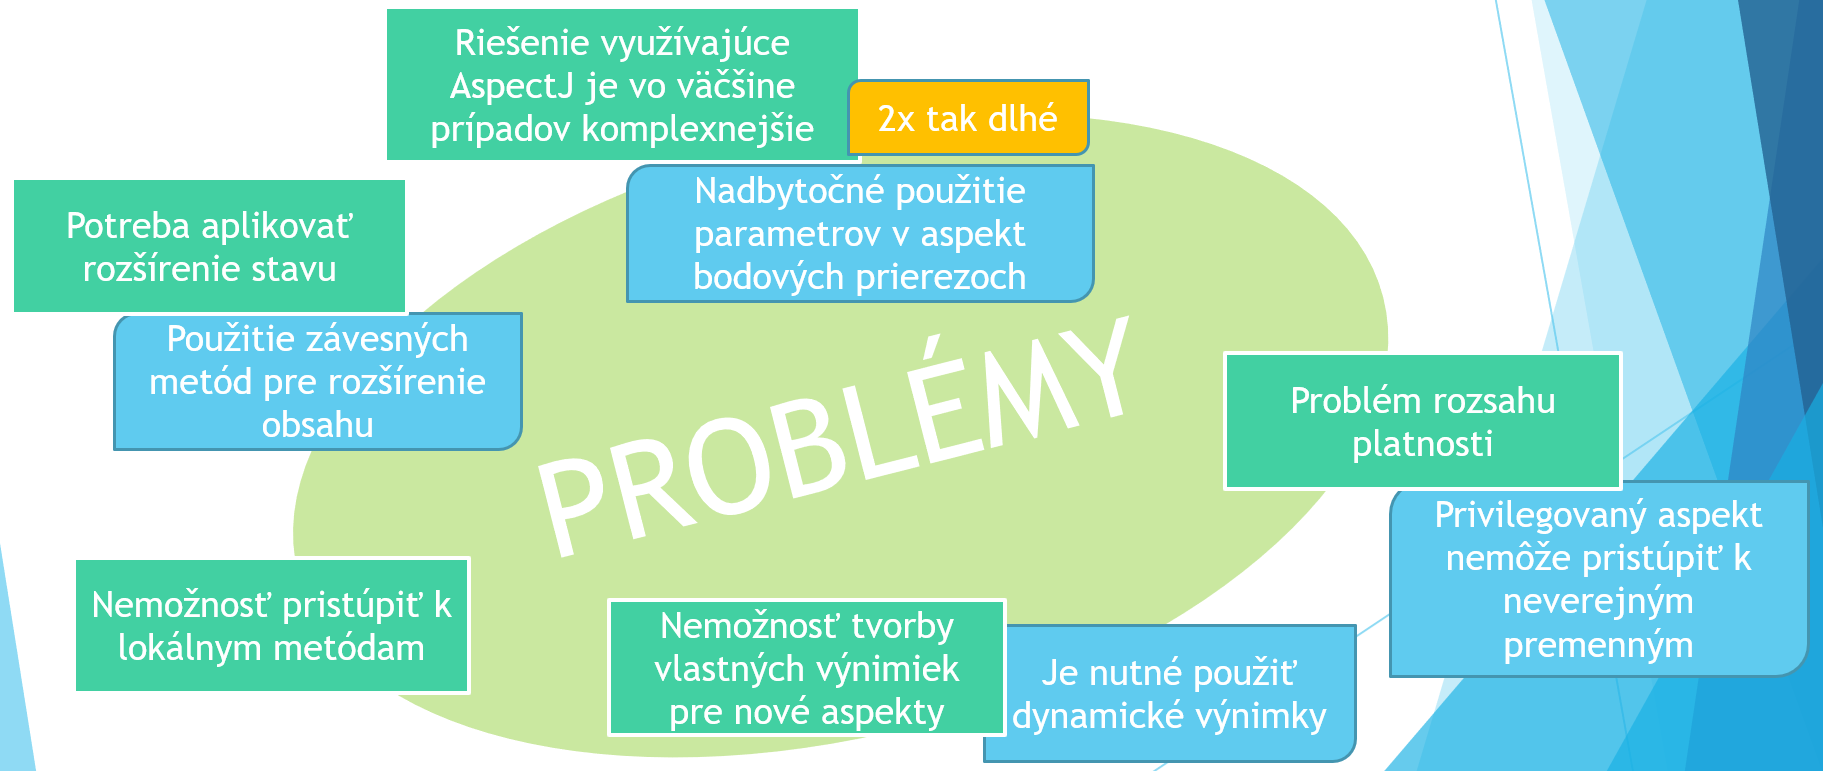
\includegraphics[width=\linewidth]{fig/problemsOfAspectJ.png}
									\caption{Problémy použitia jazyka AspectJ}
									\label{problemsOfAspectJ}
					\end{center}
\end{figure}



\section{Odvodenie konkrétnej Battleship hry} \label{layersSection}

\begin{figure}[H]  %vycentrovany obrazok grafu, vsadeny do odstavca
					\begin{center}
									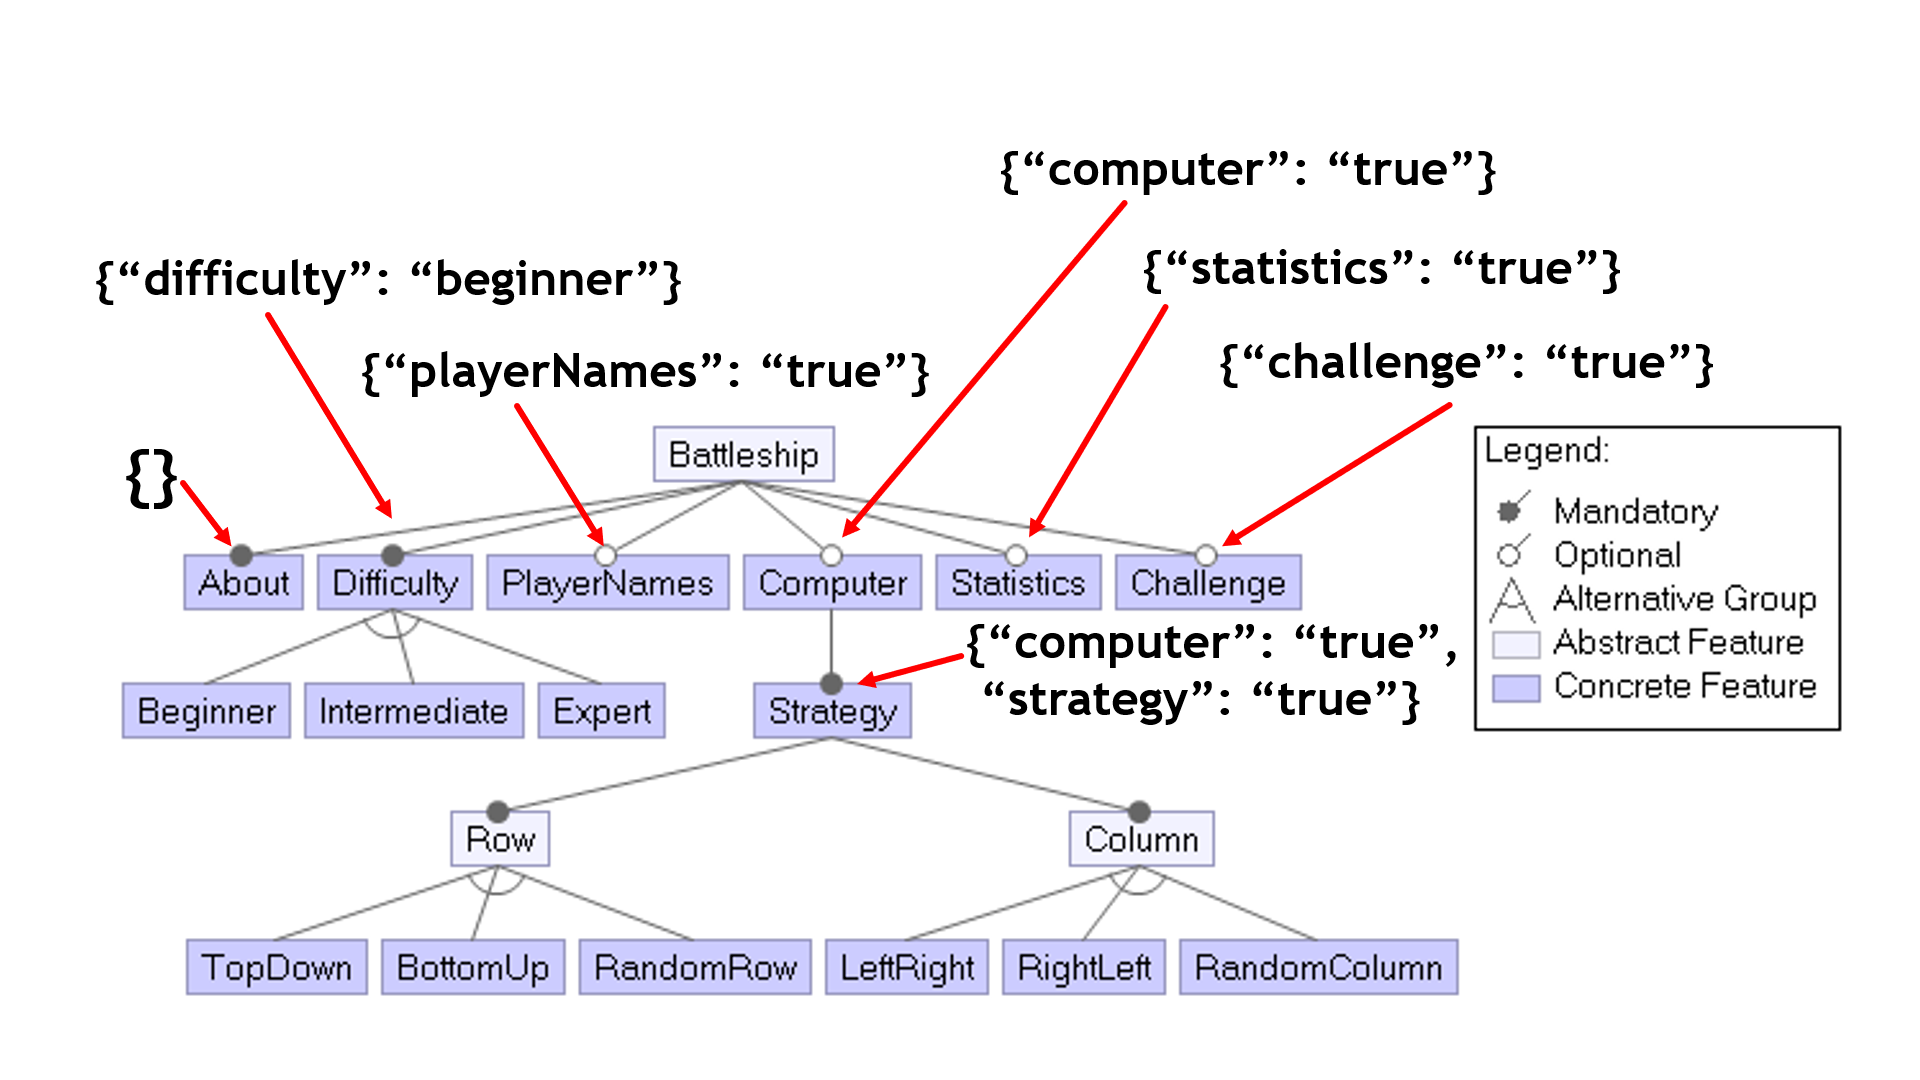
\includegraphics[width=\linewidth]{fig/derivationRules.png}
									\caption{Podoba derivačných pravidiel}
									\label{derivationRules}
					\end{center}
\end{figure}

\begin{figure}[H]  %vycentrovany obrazok grafu, vsadeny do odstavca
					\begin{center}
									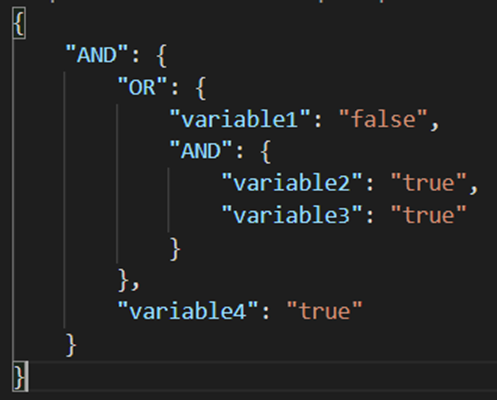
\includegraphics[width=\linewidth]{fig/expresion.png}
									\caption{Zložený derivačný výraz}
									\label{derivationRule}
					\end{center}
\end{figure}

\begin{figure}[H]  %vycentrovany obrazok grafu, vsadeny do odstavca
					\begin{center}
									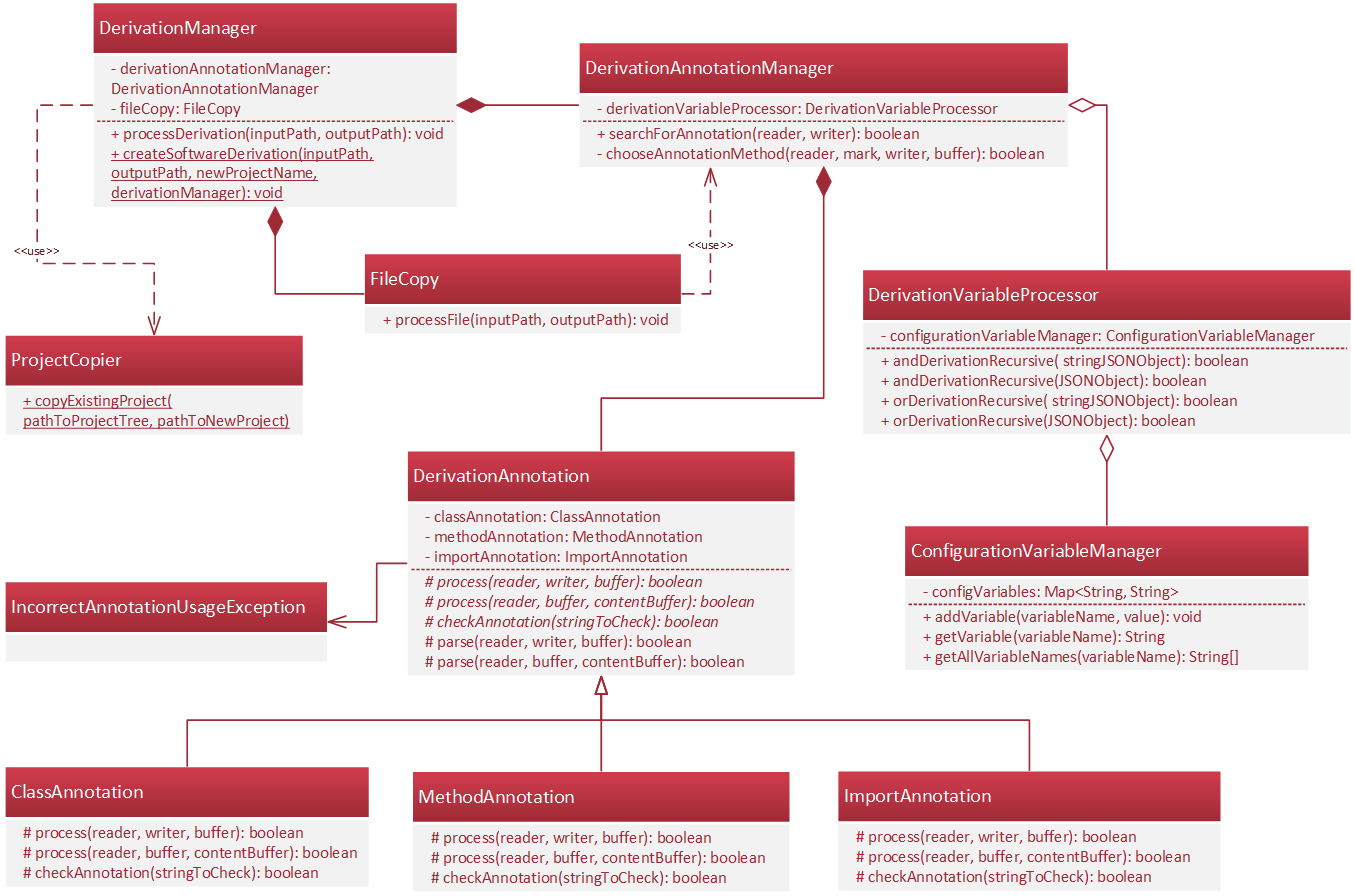
\includegraphics[width=\linewidth]{fig/DerivationClass.png}
									\caption{Diagram tried pre deriváciu produktu}
									\label{derivationProductClassDiagram}
					\end{center}
\end{figure}

\begin{figure}[H]  %vycentrovany obrazok grafu, vsadeny do odstavca
					\begin{center}
									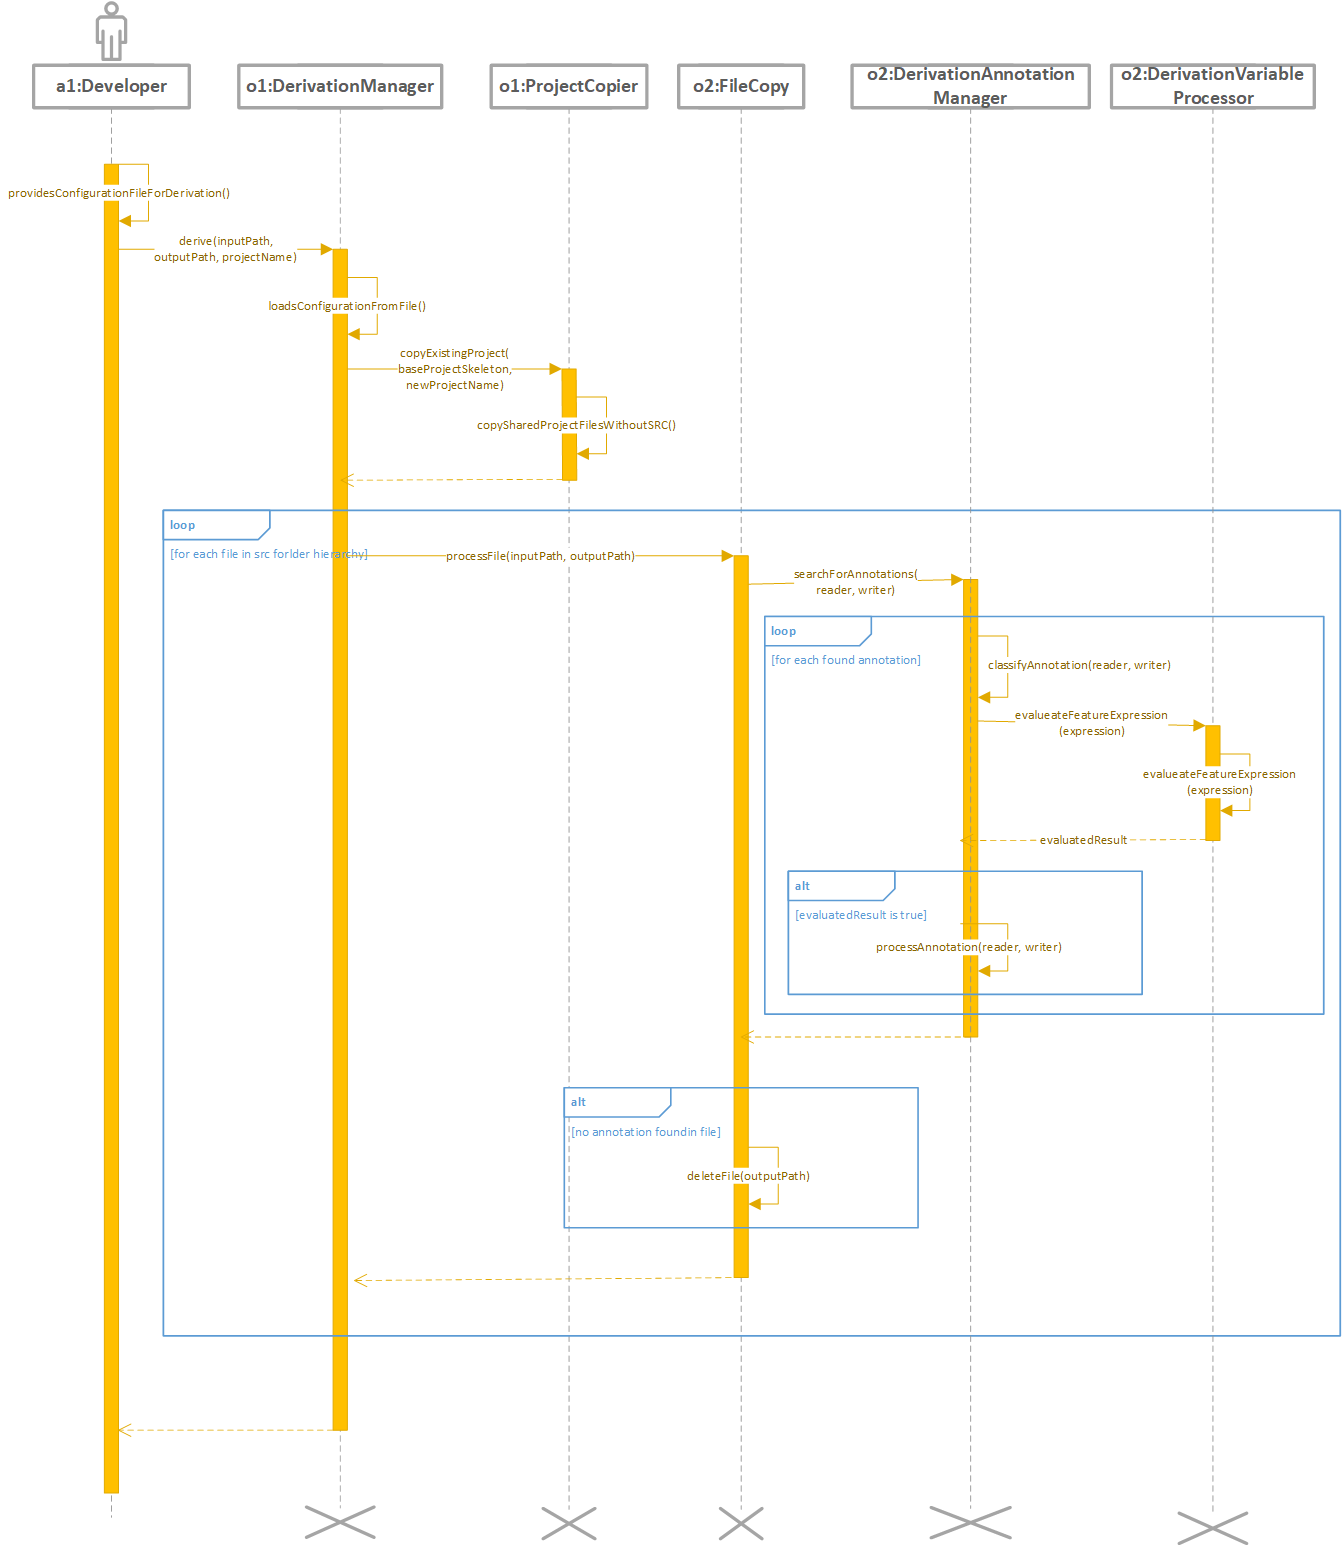
\includegraphics[width=\linewidth]{fig/derivationProcess.png}
									\caption{Sekvenčný diagram pre deriváciu produktu}
									\label{derivationProductSequenceDiagram}
					\end{center}
\end{figure}


\section{Odvodzovanie všetkých typov hier} \label{engineAsSubsystem}

Aj 

\begin{figure}[H]  %vycentrovany obrazok grafu, vsadeny do odstavca
					\begin{center}
									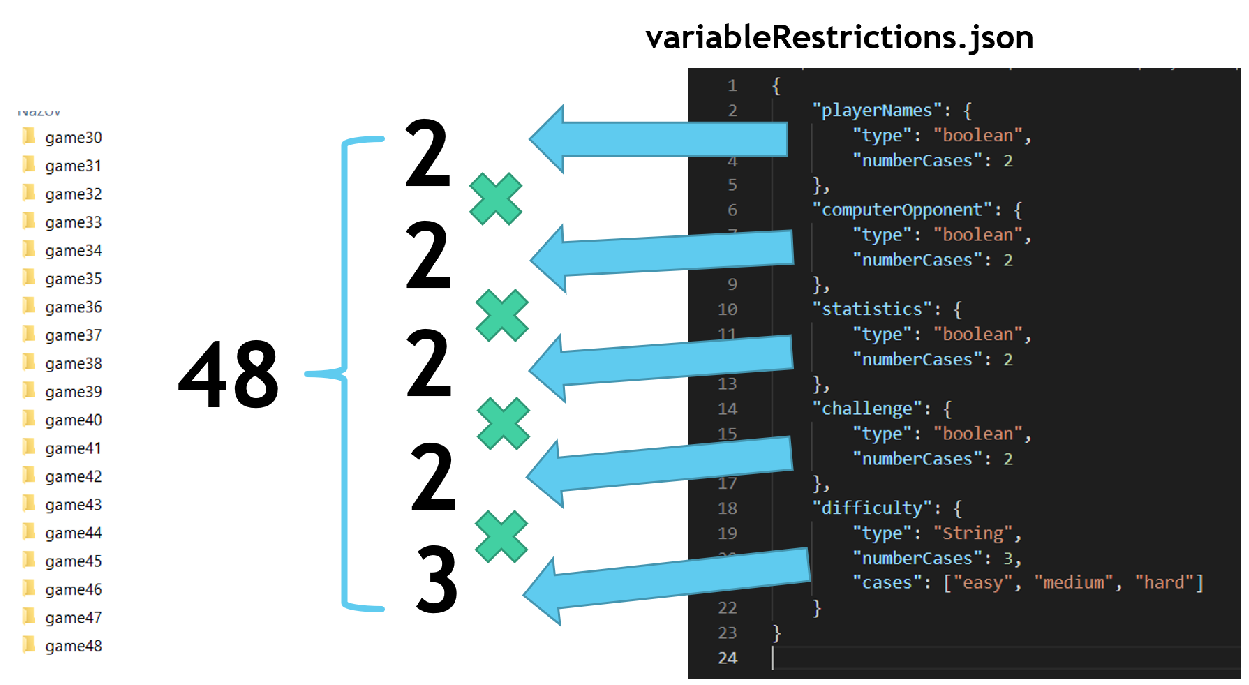
\includegraphics[width=\linewidth]{fig/allCases.png}
									\caption{Odvodenie všetkých typov hier pre hru Battleship}
									\label{derivationBattleshipTypes}
					\end{center}
\end{figure}

Kompon    



\section{Rad softvérových výrobkov pre fraktály} \label{distributedSOA}

SOA vyu\ 

\begin{figure}[H]  %vycentrovany obrazok grafu, vsadeny do odstavca
					\begin{center}
									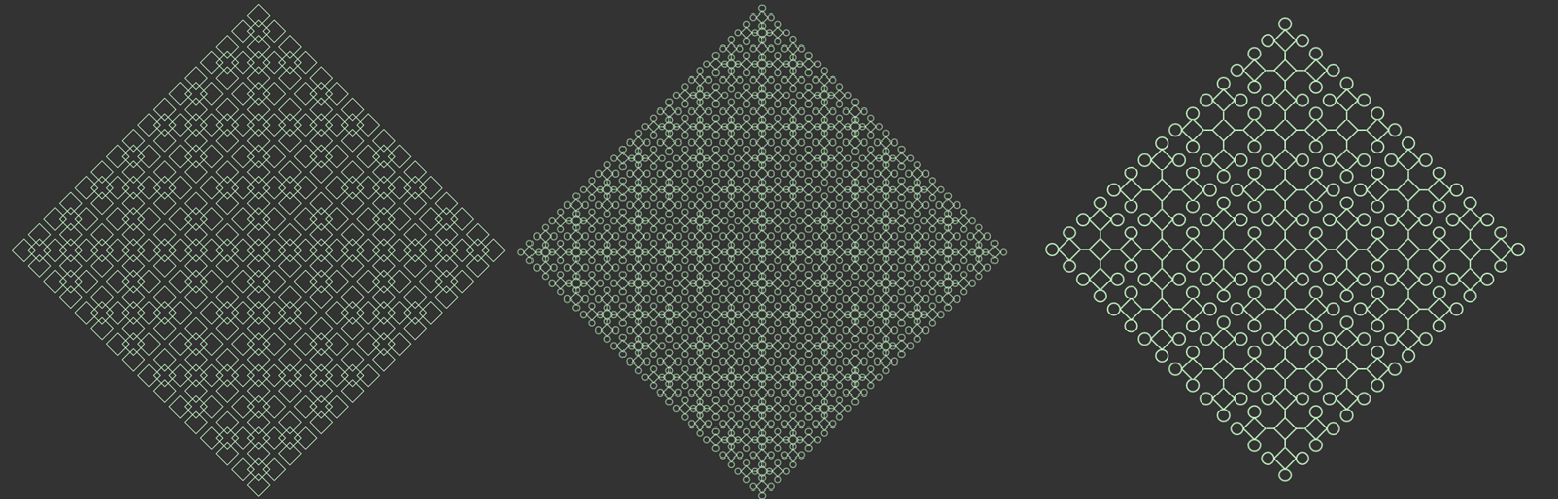
\includegraphics[width=\linewidth]{fig/fractalsAnklet.png}
									\caption{Rôzne podoby Anklet fraktálu}
									\label{ankletFractalTypes}
					\end{center}
\end{figure}

Rie\v{s}enie      


\section{Výsledná modularita a odvodené produkty} \label{eval}

Po postupn


\subsection{Úprava funkcionality a použitie jazyka AspectJ} \label{eval-ownDesing}

V návr


\subsection{Generovanie derivácií Battleship hry} \label{eval-javascript}

Vytvorili


\section{Podobná práca} \label{recentwork}

Kód kt


\section{Závery a \v{d}al\v{s}ie pokra\v{c}ovanie} \label{cc}

Analyzo
 

\bibliographystyle{abbrv} % plain or alpha are fine, too
\bibliography{bib}


\end{document}

